\section{Substitutie en parti\"ele integratie}

\subsection{Onbepaalde integraal en de kettingregel voor het afleiden}
\begin{minipage}{.25\linewidth}
	\raggedright
	
\includegraphics[width=4cm]{6_afgeleiden_integralen/inputs/QR_Code_OPPKETTINGINT_module6_3}
\end{minipage}
\begin{minipage}{.7\linewidth}
	Zie filmpje MOOC.
\end{minipage}


\subsection{Differentialen en de substitutiemethode}

Voor een functie $y=f(x)$ en $a \in \dom f$ is $Df(a)$ de richtingsco\"effici\"ent van de raaklijn $T$ aan de grafiek $G$ van $f$ in $P(a,f(a))$.
De vergelijking van de raaklijn is dan
\[
y-f(a)=Df(a).(x-a) \text { .}
\]
Het punt op die raaklijn dat behoort bij $x=a$ voldoet aan $y=f(a)$ en is dus $P(a;f(a))$ (wat logisch is).
Als je bij die $x$-waarden $\Delta x$ bijtelt dan vul je $x=a+\Delta x$ in.
Je bekomt dan de volgende waarde van $y$ op de raaklijn:
\[
y-f(a)=Df(a).(a+\Delta x -a)=Df(a).\Delta x
\]
\[
y=f(a)+Df(a).\Delta x \text { .}
\]
De verandering van de $y$-waarde op de raaklijn is dan
\[
\Delta y=Df(a).\Delta x \text { .}
\]
%\begin{figure}[h]
%	\begin{center}
%		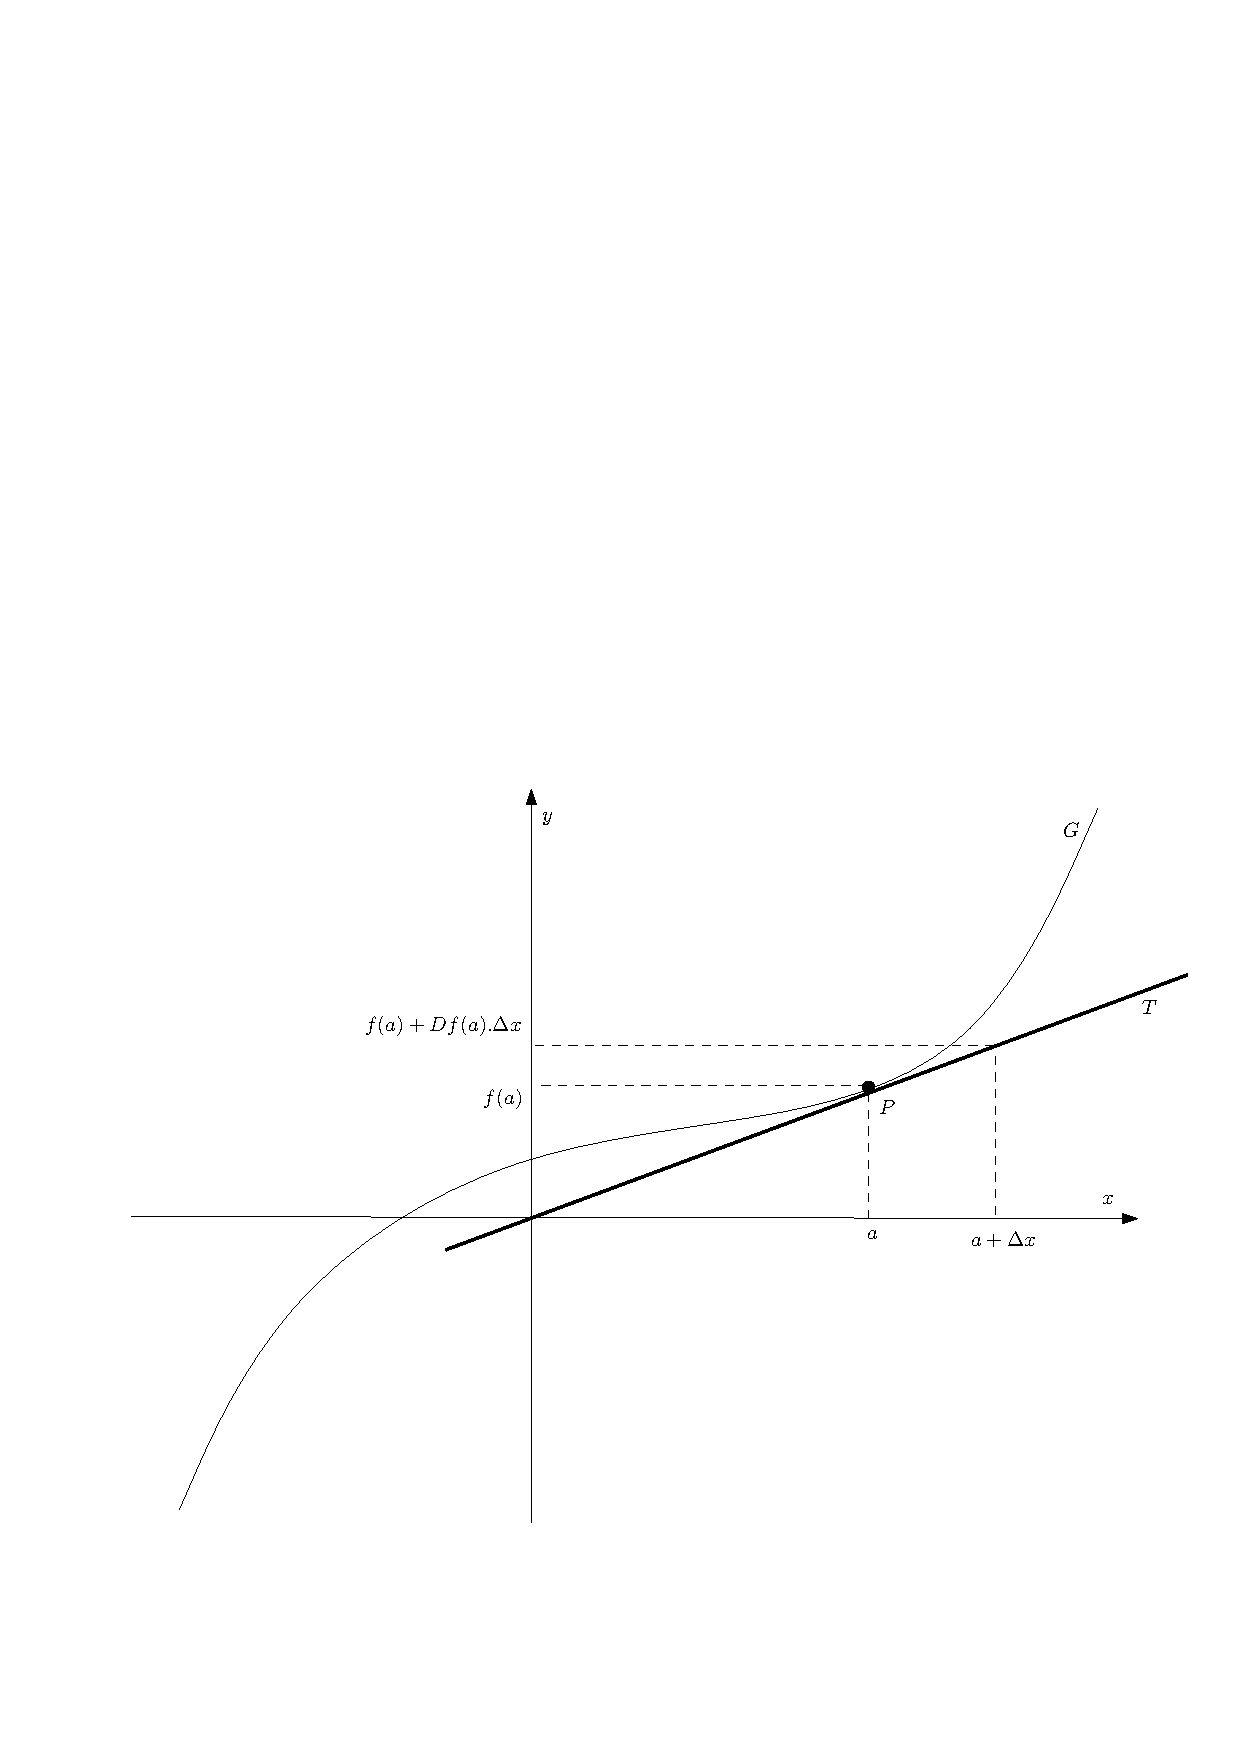
\includegraphics[height=5 cm]{6_afgeleiden_integralen/inputs/substitutie1.pdf}
%		\caption{}
%	\end{center}
%\end{figure}
Hierdoor wordt $\Delta y$ een functie in $\Delta x$ en je noemt deze functie de differentiaal van $f$ in $a$.
Je noteert  $df(a)$ voor deze functie, dus
\[
df(a)=Df(a).\Delta x \text { .}
\]
Neem je als bijzonder geval $f(x)=x$ dan is $Df(a)=1$ en dus $df(a)=\Delta x$.
Deze functie in $\Delta x$ noem je de differentiaal van $x$ en je schrijft $dx$.
Je bekomt dus
\[
dx=\Delta x \text { .}
\]
Daarom schrijft men ook
\begin{definitie}
	\[
df(a)=Df(a).dx \text { .}
\]
\end{definitie}


\begin{opmerking}
	Let wel op: het gaat hier over twee functies in de veranderlijke $\Delta x$ die een veelvoud zijn van elkaar.
\end{opmerking}

Als je de oorspronkelijke functie noteert als $y=f(x)$ dan schrijf je ook $dy(a)$ in plaats van $df(a)$.
Je bekomt dan
\[
dy(a)=Df(a).dx \text { .}
\]
Vervang je $a$ door een willekeurig getal $x$ dan schrijf je
\[
dy=Df(x).dx \text { .}
\]
Een onbepaalde integraal van een functie $y=f(x)$ genoteerd $\int f(x)dx$ kun je ook opvatten als een onbepaalde integraal van de differentiaal $f(x)dx$.\\

Uit de kettingregel voor het afleiden vinden we
\[
\int Dg(f(x))Df(x)=g(f(x))+C \text { .}
\]
Stel nu $u=f(x)$, dan is $du=Df(x)dx$ en dan bekom je
\[
\int Dg(f(x))Df(x)=\int Dg(u)du \text { .}
\]
Per definitie is $\int Dg(u)du=g(u)+C$ en door $u$ terug in te vullen vind je
\begin{definitie}
	\[
\int Dg(f(x))Df(x)dx=\int Dg(u)du=g(u)+C=g(f(x))+C \text { .}
\]
\end{definitie}

Omdat je in deze redenering $f(x)$ vervangt (substitutie) door een variabele $u$ noem je dit de methode van substitutie.
Het is gewoon een handige werkwijze om de kettingregel van het afleiden te gebruiken voor het berekenen van een onbepaalde integraal.\\

We hermaken nu de twee laatste voorbeelden uit vorig deel.\\

\begin{voorbeeld}
	$\int \sqrt[3]{x+7} dx$

Stel $u=x+7$, dan is $du=D(x+7)dx=dx$.
Je bekomt
\[
\int \sqrt[3]{x+7}dx=\int \sqrt[3]{u}du=\int u^{1/3} du=
\]
\[
=\frac{u^{4/3}}{4/3}+C=\frac{3u^{4/3}}{4}+C=\frac {3\sqrt[3]{(x+7)^4}}{4}+C \text { .}
\]

\end{voorbeeld}

%\begin{voorbeeld}
%	\noindent $\int \sin (2x-5)dx$.
%
%Stel $u=2x-5$ dan is $du=D(2x-5)dx=2dx$, dus $dx=\frac{du}{2}$.
%Je hebt
%\[
%\int \sin (2x-5)dx=\int \sin(u) \frac{du}{2}=\frac{1}{2} \int \sin (u)du=
%\]
%\[
%=-\frac{1}{2} \cos (u)+C=\frac{1}{2} \cos (2x-5)+C \text {.}
%\]
%
%\end{voorbeeld}
\vspace{2mm}

\begin{voorbeeld}
	Een iets moeilijker voorbeeld dat aantoont dat je niet steeds $dx$ moet vervangen: $\int \frac{xdx}{x^2+1}$.
\noindent (Dit lijkt mij geschikt om door middel van een filmpje te geven.)

Stel $u=x^2+1$ dan is $du=2xdx$ en dus $xdx=\frac{du}{2}$.
Je bekomt
\[
\int \frac{xdx}{x^2+1}=\int \frac{du/2}{u}=\frac{1}{2} \int \frac{du}{u}
\]
\[
=\frac{1}{2} \ln \vert u \vert +C=\frac{1}{2} \ln \left( x^2+1 \right)+C=\ln \left( \sqrt{x^2+1} \right)+C \text {.}
\]


\end{voorbeeld}

\subsection{Differentialen en de substitutiemethode - voorbeeld}
\begin{minipage}{.25\linewidth}
	\raggedright
	
\includegraphics[width=4cm]{6_afgeleiden_integralen/inputs/QR_Code_DIFFSUBSTVB_module6_3}
\end{minipage}
\begin{minipage}{.7\linewidth}
	Zie filmpje MOOC.
\end{minipage}

\subsection{Voorbeelden van de substitutiemethode}

Je leest nog enkele voorbeelden op het berekenen van integralen door middel van substitutie.

\vspace{2mm}

\begin{voorbeeld}
	$\int e^{5x}dx$
	
	Stel je $u=5x$ dan is $du=5dx$.
	
	Je vervangt dan $dx$ door $\frac{du}{5}$ en je bekomt
	\[
	\int e^{5x}dx=\int e^u\frac{du}{5}=\frac{1}{5} \int e^udu=\frac{1}{5} e^u+C=\frac{1}{5}e^{5x}+C \text { .}
	\]
	
\end{voorbeeld}

\begin{voorbeeld}
	$\int \frac{dx}{1+9x^2}$
	
	Deze integraal lijkt sterk op $\int \frac{dt}{1+t^2}=\arctan t+C$.
	
	Stel $u=3x$, dan is $du=\frac{du}{3}$ en je bekomt
	\[
	\int \frac{dx}{1+9x^2}=\int \frac{1}{1+u^2} \frac{du}{3} =\frac{1}{3} \int \frac{du}{1+u^2}=
	\]
	\[
	=\frac{1}{3} \arctan u+C=\frac{1}{3} \arctan (3x)+C \text { .}
	\]
\end{voorbeeld}
	
\begin{voorbeeld}
	$\int \frac{xdx}{\sqrt{16-x^4}}$
	
	Als je substitutie $u=16-x^4$ overweegt dan bekom je $du=-4x^3dx$.
	In de teller staat enkel $x$.
	
	De teller suggereert daarom eerder $u=x^2$ te gebruiken.
	
	Omdat je $\int \frac{dt}{\sqrt {1-t^2}}=\arcsin t+C$ kent schrijf je 
	\[
	16-x^4=16\left( 1-\frac{x^4}{16} \right)=16 \left( 1-\left( \frac{x^2}{4} \right)^2 \right) \text { .}
	\]
	De integraal die je moet oplossen is dus
	\[
	\int \frac{xdx}{\sqrt{16-x^4}}=\int \frac{xdx}{\sqrt {16 \left( 1-\left( \frac{x^2}{4} \right)^2 \right)   }}=\frac{1}{4} \int \frac{xdx}{ \sqrt{ 1-\left( \frac{x^2}{4} \right)^2   }} \text { .}
	\]
	Stel $u=\frac{x^2}{4}$, dan is $du =\frac{xdx}{2}$ en dus $xdx=2du$.
	De integraal wordt $\frac{1}{4} \int \frac{2du}{\sqrt {1-u^2}}$, dus
	\[
	\int \frac{xdx}{\sqrt{16-x^4}}=\frac{1}{2} \int \frac{du}{\sqrt {1-u^2}}=\frac{1}{2} \arcsin u+C=\frac{1}{2} \arcsin \left( \frac{x^2}{4} \right)+C \text { .}
	\]
\end{voorbeeld}
	
\begin{voorbeeld}
		$\int \frac{(\arctan x)^3dx}{1+x^2}$
	
	Stel $u=\arctan x$.
	Dan is $du=\frac{dx}{1+x^2}$ en je bekomt
	\[
	\int \frac{(\arctan x)^3dx}{1+x^2}=\int u^3du=\frac{u^4}{4}+C=\frac{(\arctan x)^4}{4}+C \text { .}
	\]
\end{voorbeeld}
	
Je merkt dat de juiste keuze maken bij substitutie wel wat oefenen vergt.

\subsection{Substitutie bij bepaalde integralen}

Stel dat je $\int ^b_a f(x)dx$ moet berekenen en dat je $\int f(x)dx$ kunt berekenen door middel van substitutie.
Als je eerst de onbepaalde integraal volledig uitrekent en daarna de grenzen invult, dan is er geen enkel probleem.
Je kunt ook in de bepaalde integraal zelf substitutie toepassen.
Je moet dan wel de grenzen aanpassen.


\begin{voorbeeld}
	$\int ^4_0 \sqrt{2x+1}dx$

Je lost eerst de onbepaalde integraal $\int \sqrt{2x+1}$ op.
Je stelt $t=2x+1$ dus $dt=2dx$ en je bekomt $\int \sqrt {2x+1} dx=\frac{1}{2} \int \sqrt {t} dt=\frac {1}{2} \frac{1}{3/2} t^{3/2}+C=\frac{1}{3} \sqrt {(2x+1)^3}+C$.
Hieruit vind je

\begin{eqnarray*}
\int ^4_0 \sqrt {2x+1} dx&=&\frac{1}{3} \left[ \sqrt {(2x+1)^3}\right] ^4_0 \\
&=&\frac{1}{3}\left( \sqrt{9^3} - \sqrt{1^3} \right)\\
&=&\frac{26}{3}
\end{eqnarray*}

Let op: $\int ^4_0 \sqrt {2x+1}dx \neq \frac{1}{2} \int ^4_0 \sqrt {t} dt$ immers $\int ^4_0 \sqrt {t} dt=\frac{3}{2}\sqrt {t^3}\vert ^4_0=\frac{3}{2}\left( \sqrt {4^3}-\sqrt {0^3} \right)=12$ en $\frac{1}{2}12=8\neq \frac{26}{3}$.

De volgende redenering is wel goed om $\int ^4_0 \sqrt {2x+1}dx$ te berekenen.
Stel $t=2x+1$ dan is $dt=2dx$ en $t=1$ als $x=0$ en $t=9$ als $x=4$.
Je bekomt

\begin{eqnarray*}
\int ^4_0 \sqrt{2x+1}dx &=& \frac{1}{2} \int ^9_1 \sqrt {t} dt \\
&=& \left[\frac{1}{2} \frac{1}{3/2} \sqrt {t^3} \right] ^9_1 \\
&=&\frac{1}{3} \left( \sqrt{9^3}-\sqrt{1^3} \right) \\
&=&\frac{26}{3}
\end{eqnarray*}

In deze laatste berekening pas je de genzen bij de substitutie aan.

\end{voorbeeld}

\subsection{Substitutie bij bepaalde integralen - voorbeeld}
\begin{minipage}{.25\linewidth}
	\raggedright
	
\includegraphics[width=4cm]{6_afgeleiden_integralen/inputs/QR_Code_SUBSTBEPVB_module6_3}
\end{minipage}
\begin{minipage}{.7\linewidth}
	Zie filmpje MOOC.
\end{minipage}


\subsection{Oefeningen op de substitutiemethode}
Je krijgt nog enkele oefeningen op het integreren door middel van substitutie.

\begin{enumerate}
	
	\item $\int \frac{dx}{\sqrt[5]{1-4x}}$
	
	\begin{itemize}
		\item Welke substitutie?
		
		Antwoord: $u=1-4x$
		\item Welke integraal bekom je dan?
		
		Antwoord: Uit $du=-4dx$ volgt $dx=-\frac{du}{4}$.
		Je bekomt
		\[
		\int \frac{dx}{\sqrt[5]{1-4x}}=-\frac{1}{4}\int \frac{du}{\sqrt[5]{u} }
		\]
		
		\item Hoe bekom je daaruit de oplossing?
		
		Antwoord: 
		\[
		-\frac{1}{4}\int \frac{du}{\sqrt[5]{u}}=-\frac{1}{4}\int u^{-1/5}du = -\frac{1}{4}\frac{u^{4/5}}{4/5}+C=-\frac{5}{16}\sqrt[5]{1-4x}+C 
		\]
		
		\item Wat is de oplossing?
		
		\[
		-\frac{5}{16}\sqrt[5]{1-4x}+C 
		\]
	\end{itemize}
	
	
	\item $\int \frac{dx}{2x-9}$
	
	\begin{itemize}
		\item Welke substitutie?
		
		Antwoord: $u=2x-9$
		
		\item Welke integraal bekom je dan?
		
		Antwoord: Uit $du=2dx$ bekom je $dx=\frac{du}{2}$.
		Je bekomt
		\[
		\int \frac{dx}{2x-9}=\frac{1}{2} \int \frac{du}{u}
		\]
		
		\item Hoe bekom je daaruit de oplossing?
		
		Antwoord:
		\[
		\frac{1}{2} \int \frac{du}{u}=\frac{1}{2} \ln \vert u \vert+C=\frac{1}{2} \ln \vert 2x-9 \vert +C
		\]
		
		\item Wat is de oplossing?
		\[
		\frac{1}{2} \ln \vert 2x-9 \vert +C
		\]
		
	\end{itemize}
	
	\item $\int \frac{x^3dx}{\sqrt{x^2+2}}$
	
	\begin{itemize}
		\item Welke substitutie?
		
		Antwoord: $t=x^2+2$
		
		\item Welke integraal bekom je dan?
		
		Antwoord: $x^3dx=\frac{1}{2}.x^2.2xdx$
		
		Omdat $t=x^2+2$ is $x^2=t-2$ en $dt=2xdx$.
		Daardoor gaat $x^3dx$ vervangen worden door $\frac{1}{2}(t-2)dt$.
		
		Bovendien wordt $\sqrt{x^2+2}$ vervangen door $\sqrt{t}$ en je bekomt
		\[
		\int \frac{x^3dx}{\sqrt{x^2+2}}=\frac{1}{2} \int \frac{t-2}{\sqrt{t}}dt
		\]
		
		\item Hoe bekom je daaruit de oplossing?
		
		\[
		\frac{1}{2} \int \frac{t-2}{\sqrt{t}}dt=\frac{1}{2} \int \frac{t}{\sqrt{t}}dt - \frac{1}{2}\int \frac{2dt}{\sqrt{t}}=
		\]
		\[
		=\frac{1}{2} \int t^{1/2}dt - \int t^{-1/2}dt=\frac{k1}{2}\frac{t^{3/2}}{3/2}-\frac{t^{1/2}}{1/2}+C=\frac{1}{3} \sqrt{(x^2+1)^3}-2\sqrt{x^2+1}+C
		\]
		
		\item Wat is de oplossing?
		\[
		\frac{1}{3} \sqrt{(x^2+1)^3}-2\sqrt{x^2+1}+C
		\]
		
	\end{itemize}
	
\end{enumerate}


\subsection{Test integraalrekening - substitutiemethode}
TODO

\subsection{Onbepaalde integralen en de productregel voor het afleiden}
\begin{minipage}{.25\linewidth}
	\raggedright
	
\includegraphics[width=4cm]{6_afgeleiden_integralen/inputs/QR_Code_ONBEPPRODUCTREGEL_module6_3}
\end{minipage}
\begin{minipage}{.7\linewidth}
	Zie filmpje MOOC.
\end{minipage}


\subsection{Methode van parti\"ele integratie}

De productregel voor het afleiden is
\[
D(f(x)g(x))=Df(x).g(x)+f(x).Dg(x) \text { .}
\]
Je kunt dit ook schrijven als
\[
f(x)Dg(x)=D(f(x)g(x))-g(x)Df(x) \text { .}
\]
Omdat per definitie $\int D(f(x)g(x))dx = f(x)g(x)+C$ bekom je hieruit \vspace{5mm}

\[
\int f(x)Dg(x)dx=f(x)g(x)-\int g(x)Df(x)dx
\]


We noteren dit met differentialen.
We stellen $u=f(x)$ en $v=g(x)$ zodat $du=Df(x)dx$ en $dv=Dg(x)dx$.
Je bekomt dan \vspace{5mm}

		\[
		\int udv=uv-\int vdu
		\]

%\begin{voorbeeld}
%	We passen dit nu toe op het beginvoorbeeld $\int x \sin x dx$.
%
%Stel $u=x$ en $dv=\sin x dx$.
%Je vindt $v$ uit $\int \sin x dx=-\cos x + C$ dus $v=-\cos x$.
%Er geldt $du = Dx .dx=dx$.
%
%Je bekomt
%\[
%\int x \sin x dx = \int udv=uv-\int vdu=
%\]
%\[
%=-x \cos x- \int -\cos x dx = -x \cos x + \int \cos x dx=- x \cos x + \sin x +C \text { .}
%\]
%\end{voorbeeld}


\begin{voorbeeld}
$\int x e^x dx$.

Stel $u=x$ en $dv=e^xdx$.
Je vindt $v$ uit $\int e^xdx=e^x+C$, dus $v=e^x$.
Er geldt $du=dx$.
Je bekomt
\[
\int xe^xdx=xe^x-\int e^xdx=xe^x-e^x+C \text { .}
\]
\vspace{2mm}

Het is belangrijk goed na te denken over de keuze van $u$ en $v$. Voor het oplossen van $\int x \sin x dx$ zou je ook volgende keuze kunnen maken:

Stel $u=\sin x$ en $dv=xdx$.
Uit $dv=xdx$ en $\int xdx = \frac{x^2}{2}+C$ bekom je $v=\frac{x^2}{2}$.
Uit $u=\sin x$ bekom je $du=\cos x dx$.
Je bekomt
\[
\int x \sin x dx=\frac{x^2}{2} \sin x-\int \frac{x^2}{2} \cos x dx \text { .}
\]
Dit is correct, maar je moet $\int x \sin x dx$ vinden en je probeert dat te doen met $\int x^2 \cos xdx$.
Deze laatste integraal is door de factor $x^2$ in plaats van de factor $x$ moeilijker dan de integraal die je wil oplossen.
Dit komt omdat je een verkeerde keuze maakt van $u$ en van $v$.
Je  moet $u$ afleiden en $v$ vind je door te integreren.
Dit moet er voor zorgen dat de integraal die je daarna nog moet uitrekenen er eenvoudiger uitziet dan de oorspronkelijke integraal.\\
\end{voorbeeld}

\begin{voorbeeld}
	$\int x^2 \ln x dx$.

Als  je $x^2$ gaat afleiden dan wordt dit $2x$; dit is eenvoudiger. 
Je moet dan wel $\ln x$ integreren maar je kent $\int \ln x dx$ mogelijk nog niet.

Als je $x^2$ gaat integreren dan wordt dit $\frac{x^3}{3}$; dit is moeilijker.
Maar je moet dan $\ln x$ afleiden en $D (\ln x) = \frac{1}{x}$.
Dit is veel eenvoudiger.

Daaruit volgt dat de laatste keuze toch de meest geschikte is.

$u=\ln x$ en dus $du=\frac{dx}{x}$.

$dv=x^2dx$ en dus $v=\frac{x^3}{3}$.

Hieruit bekom je
\[
\int x^2 \ln x dx=\frac{x^3}{3} \ln x-\int \frac{x^3}{3}\frac{1}{x}dx=
\]
\[
=\frac{x^3}{3} \ln x-\frac{1}{3} \int x^2 dx=\frac{x^3}{3} \ln x -\frac{x^3}{9}+C \text { .}
\]

\end{voorbeeld}

\subsection{Methode van parti\"ele integratie - voorbeeld 1}
\begin{minipage}{.25\linewidth}
	\raggedright
	
\includegraphics[width=4cm]{6_afgeleiden_integralen/inputs/QR_Code_PARTINTVB_module6_3}
\end{minipage}
\begin{minipage}{.7\linewidth}
	Zie filmpje MOOC.
\end{minipage}


\subsection{Methode van parti\"ele integratie - voorbeeld 2}
\begin{minipage}{.25\linewidth}
	\raggedright
	
\includegraphics[width=4cm]{6_afgeleiden_integralen/inputs/QR_Code_PARTINTVB2_module6_3}
\end{minipage}
\begin{minipage}{.7\linewidth}
	Zie filmpje MOOC.
\end{minipage}


\subsection{Voorbeelden}

Welke types van integralen kun je oplossen door gebruik te maken van parti\"ele integratie?


\begin{ftrekenregel}
	\textbf{Types:} \\

$\int x^n \sin(ax)dx$

$\int x^n \cos (ax)dx$ 

$\int x^n e^{ax}dx$ met $n \in \mathbb{N}$ en $a \in \mathbb{R}$.
\\
\\
Je neemt $u=x^n$ en $dv=\sin (ax)dx$; $dv=\cos (ax)dx$; $dv=e^{ax}dx$.\\

\end{ftrekenregel}

\begin{voorbeeld}
	$\int x^2 \cos \left( \frac{2x}{5}  \right)dx$.
	
	Neem $u=x^2$ en $dv=\cos \left( \frac{2x}{5}  \right)dx$.
	
	Dan is $du=2xdx$ en uit $\int \cos \left( \frac{2x}{5}  \right)dx=\frac{5}{2} \sin \left(  \frac{2x}{5} \right)+C$ vind je dat je $v=\frac{5}{2} \sin \left(  \frac{2x}{5} \right)$ kunt nemen.
	
	Je bekomt
	\[
	\int x^2 \cos \left( \frac{2x}{5}  \right)dx=\frac{5}{2}x^2  \sin \left(  \frac{2x}{5} \right)-5\int x  \sin \left(  \frac{2x}{5} \right)dx \text { .}
	\]
	
	Je past op de bekomen integraal opnieuw parti\"ele integratie toe.
	
	Je stelt $u=x$ en $dv= \sin \left(  \frac{2x}{5} \right)dx$.
	
	Je bekomt $du=dx$ en uit $\int  \sin \left(  \frac{2x}{5} \right)dx=-\frac{5}{2}\cos \left(  \frac{2x}{5} \right)+C$ bekom je dat je $v=-\frac{5}{2}\cos \left(  \frac{2x}{5} \right)$ kunt nemen.
	
	Je bekomt
	
	\begin{eqnarray}
		\int x  \sin \left(  \frac{2x}{5} \right)dx&=&-\frac{5}{2} x \cos \left(  \frac{2x}{5} \right)+\frac{5}{2}\int \cos \left( \frac{2x}{5}  \right)dx \\
		&=&-\frac{5}{2} x \cos \left(  \frac{2x}{5} \right)+\frac{25}{4}\sin \left( \frac{2x}{5} \right)+C
	\end{eqnarray}
	
	Voor de op te lossen integraal bekom je
	
	\begin{eqnarray*}
		\int x^2 \cos \left( \frac{2x}{5}  \right)dx &=&\frac{5}{2}x^2  \sin \left(  \frac{2x}{5} \right)-5\left( -\frac{5}{2} x \cos \left(  \frac{2x}{5} \right)+\frac{25}{4}\sin \left( \frac{2x}{5} \right)   \right)+C \\
		&=& \frac{5}{2}x^2  \sin \left(  \frac{2x}{5} \right)+\frac{25}{2} x \cos \left(  \frac{2x}{5} \right)-\frac{125}{4}\sin \left( \frac{2x}{5} \right)  +C
	\end{eqnarray*}
\end{voorbeeld}

\begin{ftrekenregel}
	
	\textbf{Types:}\\
	
	$\int x^n \ln (x)dx$
	
	$\int x^n \arcsin(ax)dx$
	
	$\int x^n \arctan(ax)dx$ met $n \in \mathbb{N}$ en $a \in \mathbb{R}$ (bij de integraal met $\ln$ mag $n \in \mathbb{R}$).
	\\
	\\
	Je neemt $u= \ln (x)$; $u=\arcsin (ax)$; $u=\arctan (ax)$ en $dv=x^n dx$.
	
	Je bekomt weliswaar $u=\frac {x^{n+1}}{n+1}$ maar omdat $dv=\frac{dx}{x}$; $dv=\frac{adx}{\sqrt{1-a^2x^2}}$; $dv=\frac {adx}{1+a^2x^2}$ bekom je daarna de integraal uit een eenvoudiger functie die je mogelijk kunt oplossen.

\end{ftrekenregel}

\begin{voorbeeld}
	
$\int x^2 \arctan(5x)dx$.

Neem $u=\arctan (5x)$ en dus $du=\frac{5dx}{1+25x^2}$ en $dv=x^2dx$ en dus $v=\frac{x^3}{3}$.

Je bekomt
\[
\int x^2 \arctan(5x)dx=\frac{x^3 \arctan (5x)}{3}-\frac{5}{3} \int \frac {x^3dx}{1+25x^2} \text { .}
\]

In de laatste integraal gebruik je substitutie $t=1+25x^2$.
Dan is $dt=50xdx$ en $x^2=\frac{t-1}{25}$.
Je bekomt

\begin{eqnarray}
\int \frac {x^3dx}{1+25x^2}&=&\frac{1}{50}\int \frac{x^2}{1+25x^2}50xdx\\
&=&\frac{1}{50}\int \frac{(t-1)/25}{t}dt \\
&=&\frac{1}{1250}\int \left( 1-\frac{1}{t}  \right)dt \\
&=&\frac{1}{1250}\left(  t-\ln \vert t \vert  \right)+C\\
&=&\frac{1}{1250} \left( 1+25x^2-\ln \left( 1+25x^2 \right) \right)
\end{eqnarray}

Voor de op te lossen integraal bekom je
\[
\int x^2 \arctan(5x)dx=\frac{x^3 \arctan (5x)}{3}-\frac{5}{3750} \left( 1+25x^2-\ln \left( 1+25x^2 \right) \right)+C \text { .}
\]

\end{voorbeeld}

\begin{voorbeeld}
	$\int \arcsin x dx$

Neem $u=\arcsin x$ dus $du=\frac{dx}{\sqrt {1-x^2}}$ en $dv=dx$ dus $v=x$.
Je bekomt
\[
\int \arcsin x dx=x \arcsin x-\int \frac{xdx}{\sqrt{1-x^2}} \text { .}
\]

In deze laatste integraal gebruik je substitutie $t=1-x^2$.
Dan is $dt=-2xdx$ en je bekomt

\begin{eqnarray*}
\int \frac{xdx}{\sqrt{1-x^2}}&=&-\frac{1}{2}\int \frac{dt}{\sqrt{t}} \\
&=&-\frac{1}{2}\frac{\sqrt{t}}{1/2}+C \\
&=&-\sqrt{t}+C \\
&=&-\sqrt{1-x^2}+C
\end{eqnarray*}

Voor de op te lossen integraal bekom je
\[
\int \arcsin x dx=x \arcsin x-\left( -\sqrt{1-x^2}  \right)+C=x \arcsin x+\sqrt{1-x^2} +C \text { .}
\]

\end{voorbeeld}


\begin{ftrekenregel}
	\textbf{Types:} \\

$\int \sin (ax)e^{bx}dx$ met $a; b \in \mathbb{R}$ (en in plaats van $\sin$ dan er ook $\cos$ staan).
\\
\\
Door tweemaal na elkaar dezelfde rollen voor $u$ en $v$ te gebruiken bekom je de som van een functie en een getal vermenigvuldigd met de te zoeken integraal.
Hieruit vind je de te zoeken integraal door het oplossen van een vergelijking.
\end{ftrekenregel}

\begin{voorbeeld}
	$\int e^{3x}\cos (5x)dx$

Stel $u=e^{3x}$ en $dv=\cos (5x)dx$.
Je bekomt $du=3e^{3x}dx$ en uit $\int \cos (5x)dx=\frac{1}{5} \sin (5x)+C$ vind je dat je $v=\frac{1}{5} \sin (5x)$ kunt nemen.
Je bekomt
\[
\int e^{3x}\cos (5x)dx=\frac{1}{5}\sin (5x)e^{3x}-\frac{3}{5}\int \sin (5x)e^{3x}dx \text { .}
\]

Stel in de nieuwe integraal opnieuw $u=e^{3x}$ en $dv=\sin (5x)dx$.
Je bekomt $du=3e^{3x}dx$ en uit $\int \sin (5x)dx=-\frac {\cos (5x)}{5}+C$ vind je dat je $v=-\frac {\cos (5x)}{5}$ kunt nemen.
Je bekomt
\[
\int \sin (5x)e^{3x}dx=-\frac {\cos (5x)e^{3x}}{5}+\frac{3}{5}\int e^{3x}\cos (5x)dx \text { .}
\]
Voor de op te lossen integraal bekom je dan

\begin{eqnarray*}
\int e^{3x}\cos (5x)dx&=&\frac{1}{5}\sin (5x)e^{3x}-\frac{3}{5} \left(  -\frac {\cos (5x)e^{3x}}{5}+\frac{3}{5}\int e^{3x}\cos (5x)dx  \right) \\
&=&\frac{1}{5}\sin (5x)e^{3x}+\frac{3}{25} \cos (5x)e^{3x}-\frac{9}{25}\int e^{3x}\cos (5x)dx 
\end{eqnarray*}


Breng je de laatste integraal over naar het linkerlid dan bekom je

\begin{equation*}
\left( 1+\frac{9}{25}  \right) \int e^{3x}\cos (5x)dx = \left(  \frac{1}{5}\sin (5x)+\frac{3}{25} \cos (5x)  \right)e^{3x}+C
\end{equation*}

Hieruit vind je

\begin{equation*}
\int e^{3x}\cos (5x)dx=\frac{25}{34} \left( \frac{1}{5}\sin (5x)+\frac{3}{25} \cos (5x)   \right)e^{3x}+C
\end{equation*}


\end{voorbeeld}

\subsection{Oefeningen}

Je krijgt nog enkele oefeningen op het berekenen van integralen door middel van parti\"ele integratie.

\begin{enumerate}
	
	\item Bereken $\int x^3e^{-5x}dx$
	
	\begin{itemize}
		\item Wat neem je voor $u$ en wat neem je voor $dv$ als je parti\"ele integratie $\int udv = uv -\int vdu$ gebruikt?
		
		Antwoord : Neem $u=x^3$ en $dv=e^{-5x}dx$.
		
		\item Wat zijn dan $du$ en $v$?
		
		Antwoord : $du=3x^2dx$ en uit $\int e^{-5x}dx=-\frac {e^{-5x}}{5} +C$ vind je dat je $v=-\frac {e^{-5x}}{5}$ kunt nemen.
		
		\item Wat bekom je als resultaat van deze partiële integratie?
		
		Antwoord : \begin{equation*}
		\int x^3e^{-5x}dx = - \frac {x^3e^{-5x}}{5}+\frac {3}{5} \int x^2e^{-5x}dx
		\end{equation*}
		
		\item Wat bekom je als je op die nieuwe integraal dezelfde soort van parti\"ele integratie toepast?
		
		Antwoord : Je stelt $u=x^2$ en dus $du=2xdx$ en opnieuw $dv=e^{-5x}dx$ en dus $v=-\frac {e^{-5x}}{5}$.
		Je bekomt \begin{equation*}
		\int x^2e^{-5x}dx =  - \frac {x^2e^{-5x}}{5}+\frac {2}{5} \int xe^{-5x}dx
		\end{equation*}
		
		\item Wat bekom je als je op die nieuwe integraal nogmaals parti\"ele integratie toepast?
		
		Antwoord : \begin{equation*}
		\int xe^{-5x}dx = - \frac {xe^{-5x}}{5}+\frac {1}{5} \int e^{-5x}dx= - \frac {xe^{-5x}}{5}-\frac{1}{25}e^{-5x}+C
		\end{equation*}
		
		\item Wat bekom je voor de integraal die je moet oplossen?
		
		Antwoord : \begin{equation*}
		\int x^3e{-5x}dx = - \frac {x^3e^{-5x}}{5}+\frac {3}{5} \left(  - \frac {x^2e^{-5x}}{5}+\frac {2}{5} \left( - \frac {xe^{-5x}}{5}-\frac{1}{25}e^{-5x}+C  \right)   \right)+C
		\end{equation*}
		
		
		\item Wat is de oplossing?
		
		Antwoord : \begin{equation*}
		\int x^3e^{-5x}dx = \left( -\frac{x^3}{5}-\frac{3x^2}{25}-\frac{6x}{125}-\frac{6}{625}   \right)e^{-5x}+C
		\end{equation*}
		
	\end{itemize}
	
	\item Bereken $\int \sqrt[3]{x^5} \ln x dx$
	
	\begin{itemize}
		
		\item Wat neem je voor $u$ en wat neem je voor $dv$ als je parti\"ele integratie $\int udv = uv -\int vdu$ gebruikt?
		
		Antwoord : Neem $u= \ln x$ en $dv=\sqrt[3]{x^5}dx$ .
		
		\item Wat zijn dan $du$ en $v$?
		
		Antwoord : $du=\frac{dx}{x}$ en uit $\int \sqrt[3]{x^5}dx=\int x^{5/3}dx=\frac{x^{8/3}}{8/3}+C$ bekom je dat je kan nemen $v=\frac{3x^{8/3}}{8}$.
		
		\item Wat bekom je als resultaat van deze parti\"ele integratie?
		
		Antwoord : \begin{equation*}
		\int \sqrt[3]{x^5} \ln x dx=\frac{3x^{8/3}}{8} \ln x-\frac{3}{8}\int x^{8/3}\frac{1}{x}dx
		\end{equation*}
		
		\item Wat bekom je als oplossing van die nieuwe integraal?
		
		Antwoord : \begin{equation*}
		\int x^{8/3}\frac{1}{x}dx=\int x^{5/3}dx=\frac{x^{8/3}}{8/3}+C=\frac{3x^{8/3}}{8}+C
		\end{equation*}
		
		\item Wat bekom je voor de integraal die je moet oplossen?
		
		Antwoord :  \begin{equation*}
		\int \sqrt[3]{x^5} \ln x dx=\frac{3x^{8/3}}{8} \ln x-\frac{3}{8}\left( \frac{3x^{8/3}}{8}  \right)+C
		\end{equation*}
		
		\item Wat is de oplossing?
		
		Antwoord :  \begin{equation*}
		\int \sqrt[3]{x^5} \ln x dx= \frac{3}{8} \sqrt[3]{x^8} \left( \ln x -\frac {3}{8}  \right) +C
		\end{equation*}
		
	\end{itemize}
	
	\item Bereken $\int e^{-x/2}\sin \left( \frac{x}{3}  \right)dx$
	
	\begin{itemize}
		
		\item Wat neem je voor $u$ en wat neem je voor $dv$ als je parti\"ele integratie $\int udv = uv -\int vdu$ gebruikt?
		
		Antwoord : Neem $u=e^{-x/2}$ en $dv=\sin \left( \frac{x}{3}  \right)dx$ (je mag ook $u=\sin \left( \frac{x}{3}  \right)$ en $dv=e^{-x/2}dx$ nemen).
		
		\item Wat zijn dan $du$ en $v$?
		
		Antwoord : $du=-\frac{e^{-x/2}}{2}dx$ en uit $\int \sin \left( \frac{x}{3}  \right)dx=-3 \cos \left( \frac{x}{3}  \right)+C$ vind je dat je $v=-3 \cos \left( \frac{x}{3}  \right)$ kan nemen.
		
		\item Wat bekom je als resultaat van deze parti\"ele integratie?
		
		Antwoord :  \begin{equation*}
		\int e^{-x/2}\sin \left( \frac{x}{3}  \right)dx=-3e^{-x/2} \cos \left( \frac{x}{3}  \right)-\frac{3}{2} \int e^{-x/2}\cos \left( \frac{x}{3}  \right)dx
		\end{equation*}
		
		\item Wat bekom je als je op die nieuwe integraal dezelfde soort van parti\"ele integratie toepast?
		
		Antwoord: Je neemt opnieuw $u=e^{-x/2}$ en dus $du=-\frac{e^{-x/2}}{2}dx$ en $dv=\cos \left( \frac{x}{3}  \right)dx$ waaruit je bekomt \begin{equation*}
		v=3 \sin \left( \frac{x}{3}  \right)
		\end{equation*}
		Je bekomt \begin{equation*}
		\int e^{-x/2}\cos \left( \frac{x}{3}  \right)dx=3e^{-x/2}\sin \left( \frac{x}{3}  \right)+\frac{3}{2}\int e^{-x/2}\sin \left( \frac{x}{3}  \right)dx
		\end{equation*}
		
		\item Wat bekom je voor de integraal die je moet oplossen?
		
		Antwoord: \begin{equation*}
		\int e^{-x/2}\sin \left( \frac{x}{3}  \right)dx=-3e^{-x/2} \cos \left( \frac{x}{3}  \right)-\frac{3}{2} \left(  3e^{-x/2}\sin \left( \frac{x}{3}  \right)+\frac{3}{2}\int e^{-x/2}\sin \left( \frac{x}{3}  \right)dx \right)
		\end{equation*}
		
		\item Wat bekom je als je de integraal in het rechterlid mee naar het linkerlid brengt?
		
		Antwoord : \begin{equation*}
		\left(  1+\frac{9}{4} \right)\int e^{-x/2}\sin \left( \frac{x}{3}  \right)dx=-3e^{-x/2} \cos \left( \frac{x}{3}  \right)-\frac{9}{2} e^{-x/2}\sin \left( \frac{x}{3}  \right)+C
		\end{equation*}
		
		\item Wat is de oplossing?
		
		Antwoord: 
		\begin{equation*}
		\int e^{-x/2}\sin \left( \frac{x}{3}  \right)dx=\frac{4}{13}e^{-x/2} \left( -3 \cos \left( 	\frac{x}{3}  \right)-\frac{9}{2}\sin \left( \frac{x}{3}  \right) \right)+C
		\end{equation*}
		
	\end{itemize}
	
\end{enumerate}


\subsection{Parti\"ele integratie bij bepaalde integralen}

Je kunt parti\"ele integratie onmiddellijk toepassen bij bepaalde integralen zoals in volgend voorbeeld.

\begin{eqnarray*}
\int ^e_1 \ln x dx &=& \left[ x \cdot \ln x \right] ^e_1- \int ^e_1 x d(\ln x) \\
&=& \left[ x \cdot \ln x \right] ^e_1-\int ^e_1dx \\
&=& \left[ x \cdot \ln x -x \right] ^e_1 \\
&=&
e.\ln e - e - (1.\ln 1 -1)=1
\end{eqnarray*}

Denk er aan dat je ook in het deel $vu$ van de regel $\int udv=uv+\int vdu$ de grenzen moet invullen. Als je dat vergeet dan bekom je als uitkomst van een bepaalde integraal immers een functievoorschrift terwijl het resultaat van een bepaalde integraal een getal moet zijn.


\subsection{Test integraalrekening - parti\"ele integratie}
TODO